\documentclass[]{beamer}

\usepackage[ngerman]{babel}
\usepackage[utf8]{inputenc}
\usepackage{amsmath,amsfonts,amssymb}

\usetheme{Frankfurt}
\usecolortheme{default} % % beaver
\usefonttheme{default}
\useinnertheme{rounded} % % default
\useoutertheme{default}
\usepackage{graphicx}

\title{How NAO learns to kick the ball ...}
\author{Jannick, André, Daniel, Florian}
\date{11.07.2012}
\titlegraphic{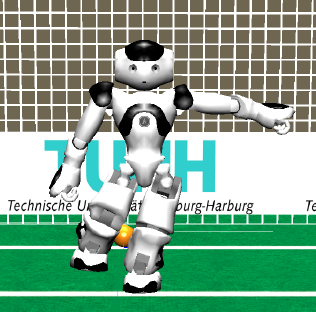
\includegraphics[scale=0.45]{nao3}}

\begin{document}

%% frame 1
\begin{frame}
	\titlepage
\end{frame}
%% frame 1

\section*{Agenda}
%% frame 2
\begin{frame}
	\frametitle{Agenda}
  	\tableofcontents
\end{frame}
%% frame 2

\section{Einleitung}
%% frame 3
\begin{frame}
	\frametitle{Einleitung}
	\begin{itemize}
		\item Arbeit mit Robotiksystemen
		\item Implementieren einer Schussbewegung für NAO
	\end{itemize}		
\end{frame}
%% frame 3

\section{Arbeitsschritte}
%% frame 4
\begin{frame}
	\frametitle{Arbeitsschritte}
	\begin{enumerate}
		\item Statisches Gleichgewicht auf einem Bein (Simulator)
		\item Vollführen einer Schussbewegung (Simulator)
		\item "'Übertragen"' auf den NAO (Simulator, NAO)
	\end{enumerate}
\end{frame}
%% frame 4

\subsection{Phase 1}
%% frame 5a
\begin{frame}
	\frametitle{Phase 1 - Schwerpunkt}
	\begin{itemize}
		\item Einarbeiten in die API und Nutzung des Simulators Webots (naoController.m)
		\item Verschieben des Schwerpunktes über linkes Bein (ForwardKinematics, InverseKinematics)
		\item Anheben des rechten Fußes	
	\end{itemize}
	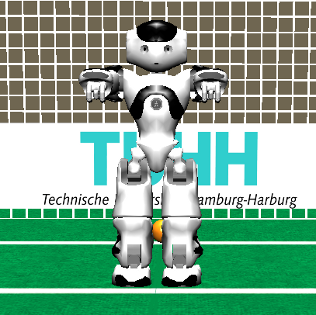
\includegraphics[width=3.3cm]{nao1}
	\includegraphics[scale=0.3]{space}
	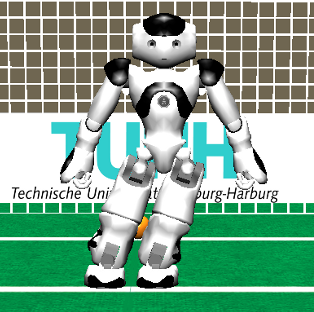
\includegraphics[width=3.3cm]{nao2}
	\includegraphics[scale=0.3]{space}
	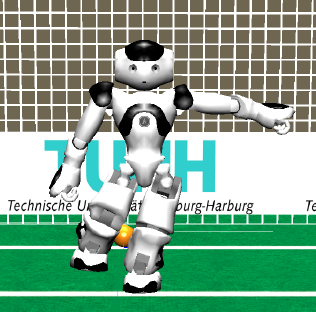
\includegraphics[width=3.3cm]{nao3}
\end{frame}
%% frame 5a 

% % frame 5b 
\begin{frame}
	\frametitle{Schwerpunktverschiebung}
	\begin{columns}

		\column{0.3\textwidth}
		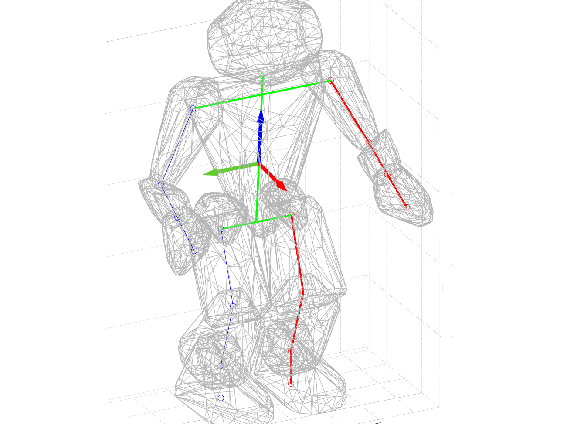
\includegraphics[width=4.7cm]{comtorso}
		\newline\newline
		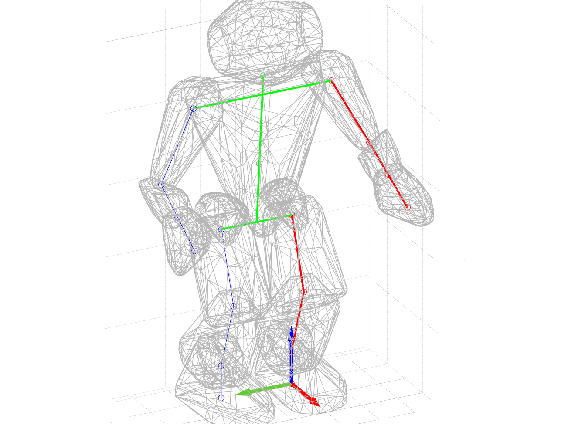
\includegraphics[width=4.7cm]{comfoot}
		
		\column{0.7\textwidth}
		Pseudo-Code:
		\newline\newline
		%% Aus dem blackboard holen
		$get: KinematicMatrix$ $XFoot$
		$get: KinematicMatrix$ $Com2Torso$
		\newline\newline
		$Torso2XFoot = XFoot^{-1}$	
		$Com2XFoot = Torso2XFoot \cdot Com2Torso$					
		\newline\newline
		$set$ $y$ $and$ $x$ $coordinates$
		\newline\newline
		$XFoot2Com = Com2XFoot^{-1}$
		$XFoot = Com2Torso * XFoot2Com$
		\newline\newline
		$get$ $angles$ $via$ $InverseKinematics$
	\end{columns}
\end{frame}
% % frame 5b

\subsection{Phase 2}
%% frame 6a
\begin{frame}
	\frametitle{Phase 2 - Schuss}
	\begin{itemize}
		\item Ausgangslage:
		\begin{itemize}
			\item Ball liegt vor der Fußspitze des NAOs
		\end{itemize} 		 
		\item Die Frage nach dem "Wie" der Schussbewegung
		\item Ziele:
		\begin{itemize}
			\item Ball auf mittlerer Höhe treffen
			\item Nicht umfallen
			\item Einen großen Impuls übertragen
			\item Keine innere Kollision
			%% Wie hatten wir das hier nochmal gelöst?
			\item Einstellen des Schusswinkels
		\end{itemize}		 		 
	\end{itemize}
\end{frame}
%% frame 6a

%% frame 6b
\begin{frame}
	\frametitle{Einstellen des Schusswinkels und der Fußposition}
	\begin{center}
	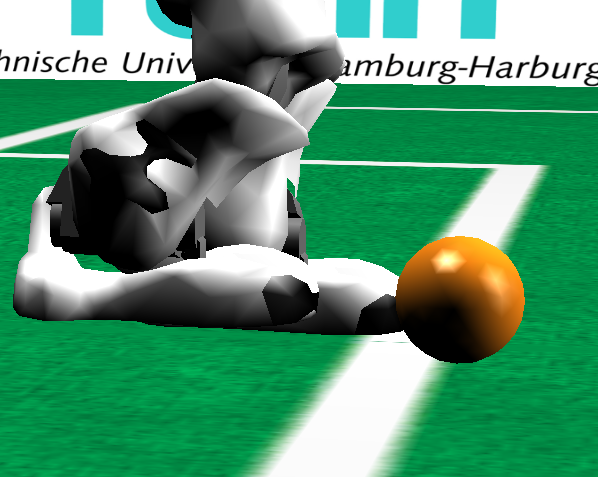
\includegraphics[width=3.3cm]{shootside}
	\includegraphics[scale=0.3]{space}
	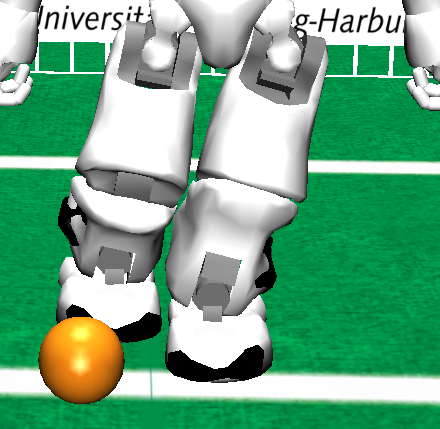
\includegraphics[width=3.3cm]{shootfrontinner}
	\includegraphics[scale=0.3]{space}
	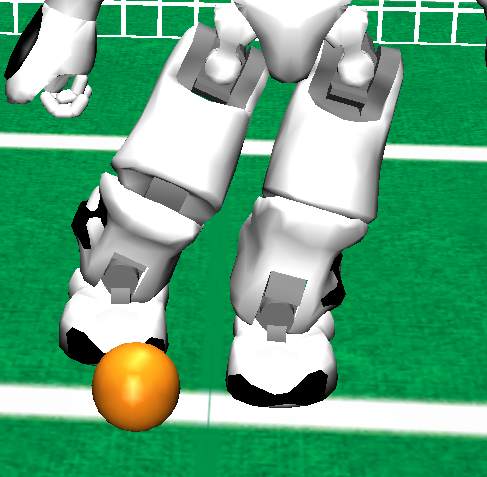
\includegraphics[width=3.3cm]{shhotfrontouter}
	\end{center}
\end{frame}
%% frame 6b 

\subsection{Phase 3}
%% frame 7
\begin{frame}
	\frametitle{Phase 3 - Schuss optimieren und übertragen auf den NAO}
	\begin{itemize}
		\item Übertragen des naoController (Matlab) in C++
		\item Test auf dem Roboter
		\item Idee: Genauere Schusswinkeleinstellung (Interpolation der Fußform), aber Praxistest zeigt, dass noch weitere Parameter wichtig sind.
	\end{itemize}
\end{frame}
%% frame 7	

\section{Ergebnis und Ausblick}
%% frame 8
\begin{frame}
	\frametitle{Ergebnis und Ausblick}
	\begin{itemize}
		\item TuhhSDK und vorhandene Projektstruktur erleichtern Einarbeitung
		\item Implementierung der Schussbewegung als einzelnes Modul
		\item Eingeschränkter Schusswinkel
		\item Nächster nötiger Arbeitsschritt: genauere Schusswinkelbestimmung (und erkennen, annähern und positionieren vor dem Ball)  
	\end{itemize}
\end{frame}
%% frame 8

\section{Präsentation}	
%% frame 9
\begin{frame}
	\frametitle{Präsentation}
	\begin{center}
		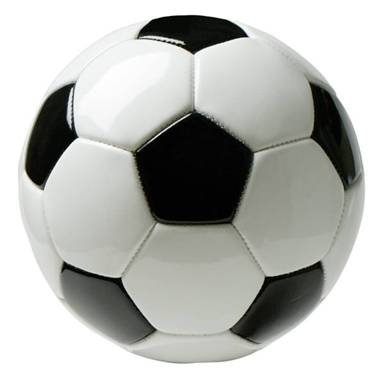
\includegraphics[scale=0.5]{football}
	\end{center}
\end{frame}
%% frame 9
	
\end{document}